% Feature Model of the tsam aggregation configuration — VERSION 2.
%
% This is feature_model.tex plus ONE addition: every group is tagged with the
% configuration object that owns it. feature_model.tex is left untouched so the
% two can be compared and either kept.
%
% Notation: FODA feature diagram (Kang et al., CMU/SEI-90-TR-21, 1990):
%   filled circle on an edge   = MANDATORY feature
%   open circle on an edge     = OPTIONAL feature
%   unfilled arc across a fan  = ALTERNATIVE group (choose EXACTLY ONE)
%   filled arc across a fan    = OR group (choose ONE OR MORE)
%   dashed arrow               = cross-tree constraint (requires)
%
% ── WHAT V2 ADDS: THE OWNER TAG ───────────────────────────────────────────
% A feature model says what can be chosen but not where to type it. Each group
% box now carries a third line, in \ttfamily, naming the object that owns those
% options. Verified against src/tsam/api.py:25-38 and src/tsam/config.py:
%
%   Weighting       ClusterConfig  — scale_by_column_means, use_duration_curves,
%                                    include_period_sums
%                   aggregate()    — weights   <- the one exception, see below
%   Grouping        ClusterConfig.method
%   Representation  ClusterConfig.representation
%   Extreme periods ExtremeConfig.method
%   Rescaling       aggregate()    — preserve_column_means, rescale_exclude_columns
%   Segmentation    SegmentConfig  — n_segments, representation
%
% THE RULE FOR WHERE A TAG GOES: the group box carries the owner of its
% features; a LEAF carries its own tag only when it differs from its group's.
% Exactly one leaf differs today — `weights` is an aggregate() keyword while
% the rest of the Weighting group are ClusterConfig fields — so it is the only
% tagged leaf. Tagging all four leaves instead would need three lines in each
% of the other three boxes, which does not fit the row pitch.
%
% Only the class name is given, not class.attribute: the question the tag
% answers is "which object do I construct", and `ClusterConfig.representation`
% sets 26 mm at \tiny \ttfamily against 21.5 mm of text width.
%
% Distribution's own parameters (band 2) are not tagged: the band root says
% Distribution, so repeating it on all three groups would break the
% say-the-stereotype-once rule. That Distribution is itself a value of
% ClusterConfig.representation / SegmentConfig.representation belongs in the
% caption — adding it to the band-2 root costs 3 mm and pushes the aspect to
% 1.254, over budget.
%
% ── PRINT TARGET ──────────────────────────────────────────────────────────
% Text column 165.1 x 228.6 mm, figures at full width: ASPECT h/w <= 1.24 and
% WIDTH <= ~165 mm. The taller group boxes are paid for by dropping the band-1
% leaf pitch from 10 mm to 9.5 mm; this lands at ~164.7 x ~203.5 mm,
% aspect ~1.236. There is no slack left — re-measure if anything is added.
%
% ── LAYOUT GRID (millimetres, y negative downwards) ───────────────────────
% BAND 1 — six columns, pitch 27, boxes 24.5 mm wide:
%   c1 = 17 Weighting   c2 = 44 Grouping     c3 = 71 Representation
%   c4 = 98 Extremes    c5 = 125 Rescaling   c6 = 152 Segmentation
%   root (84.5,-8) 44x9   bar y -18   markers y -20.7
%   groups y -24..-37 (13 mm, up from 11 to hold the owner line)
%   leaf bus x = ci-15, elbow y -40, stub ci-15 -> ci-10.5
%   leaves 21 mm wide, rows -48 -57.5 -67 -76.5 -86 -95.5 (pitch 9.5)
%   arcs: x radius 3 at (ci-10.5, first row), y radius = half the row span
% CONNECTOR to band 2: (81.5,-76.5) -- (86,-76.5) -- (86,-106).
% BAND 2 — three columns, pitch 53, boxes 44 mm wide:
%   c1 = 30 scope   c2 = 83 concurrency   c3 = 136 preserve_minmax
%   root (84.5,-110.5) 44x9   bar y -121   markers y -123.5
%   groups y -126.5..-137.5   leaf bus x = ci-27, elbow y -141
%   leaves 40 mm wide, rows -148 -157 -166 -175 -184 (pitch 9)
%   constraint lane x = 53.5: clears c1's group (ends 52) by 1.5 mm and c2's
%     bus (56) by 2.5 mm, and passes both elbows at y -141 outside their
%     x-ranges.
%
% ── TRAPS RE-CHECKED HERE ─────────────────────────────────────────────────
%   * A TikZ node CLIPS NOTHING and LaTeX will not break at `\_`, so long
%     snake_case leaves are broken by hand. MEASURED widths at \tiny:
%       ClusterConfig \ttfamily 12.1 mm    aggregate() \ttfamily 10.2 mm
%     both inside the 21.5 mm group text width.
%   * `minimum height` is a MINIMUM: a three-line leaf grows its own box, so
%     the row pitch, not the box height, has to leave the gap. At pitch 9.5
%     with 8 mm boxes that gap is 1.5 mm, which two-line leaves still clear.
%   * A TikZ STYLE cannot be applied to part of a node's text; the phase and
%     owner tags use \newcommand DECLARATIONS.
%   * NEVER sed this file — use an editor. A `s/\\wd/.../` pattern once
%     rewrote every bare "wd", turning \newcommand into \newcommamywd.
%
% Regenerate:
%   tectonic feature_model_v2.tex
%   pdftocairo -svg feature_model_v2.pdf feature_model_v2.svg

\documentclass[10pt,border=1mm]{standalone}
\usepackage[T1]{fontenc}
\usepackage{lmodern}
\usepackage{tikz}
\usetikzlibrary{positioning,arrows.meta,fit,backgrounds,calc}

\definecolor{fzjblue}{HTML}{023D6B}
\definecolor{fzjdark}{HTML}{012845}
\definecolor{tintblue}{HTML}{DCE9F2}
\definecolor{amber}{HTML}{A8681A}
\definecolor{ambertint}{HTML}{FBF1E4}
\definecolor{greytext}{HTML}{3F4A55}

% DECLARATIONS, not TikZ styles: a style cannot be applied to part of a node's
% text, which is what the phase tag and the owner tag both need.
\newcommand{\ph}{\tiny\color{greytext}}
\newcommand{\ow}{\tiny\ttfamily\color{fzjdark}}

\begin{document}
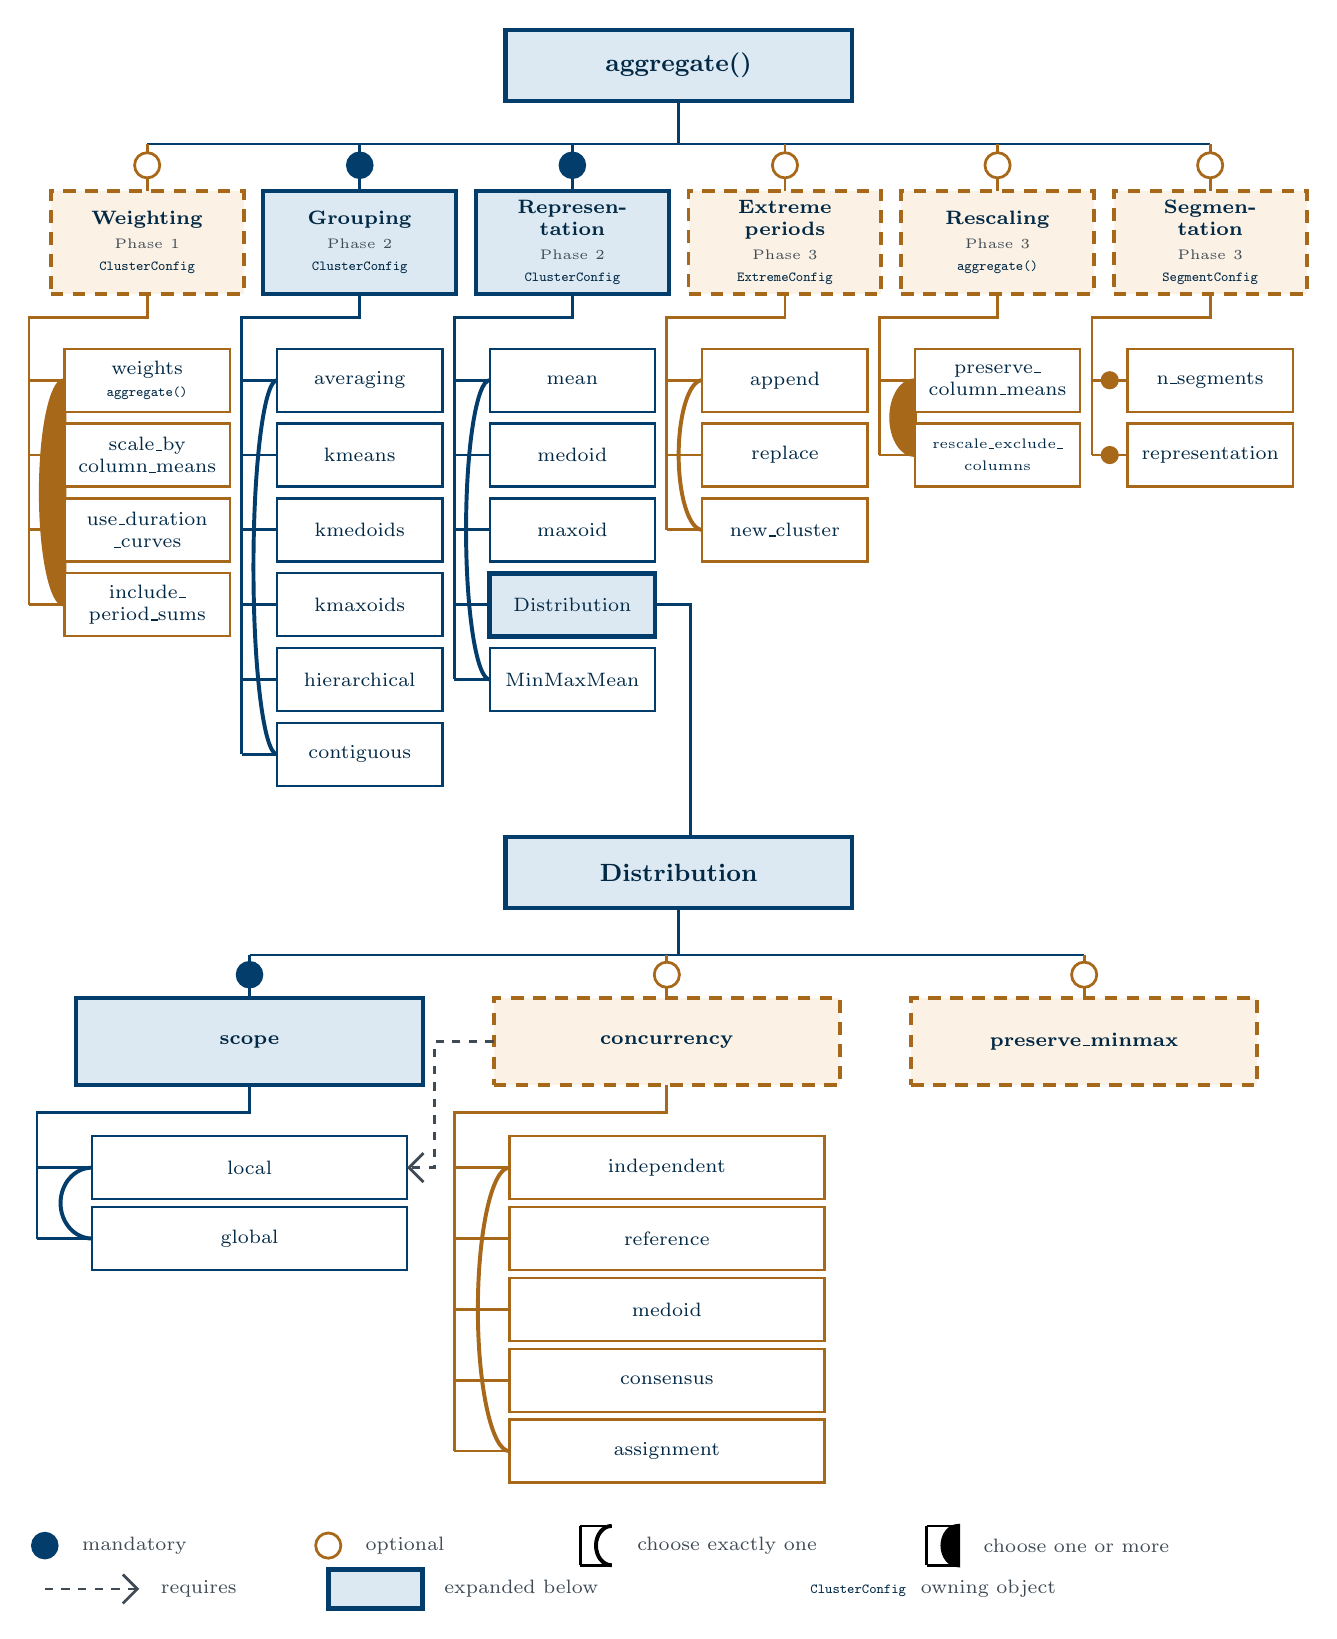
\begin{tikzpicture}[
  x=1mm, y=1mm,
  root/.style={
    draw=fzjblue, line width=0.55mm, fill=tintblue, text=fzjdark,
    minimum width=44mm, minimum height=9mm, text width=40mm,
    align=center, font=\small\bfseries},
  grpm/.style={
    draw=fzjblue, line width=0.5mm, fill=tintblue, text=fzjdark,
    minimum width=24.5mm, minimum height=13mm, text width=21.5mm,
    align=center, font=\scriptsize},
  grpo/.style={
    draw=amber, line width=0.5mm, dash pattern=on 1.6mm off 1.2mm,
    fill=ambertint, text=fzjdark,
    minimum width=24.5mm, minimum height=13mm, text width=21.5mm,
    align=center, font=\scriptsize},
  leaf/.style={
    draw=fzjblue, line width=0.3mm, fill=white, text=fzjdark,
    minimum width=21mm, minimum height=8mm, text width=18.5mm,
    align=center, font=\scriptsize},
  leafo/.style={
    draw=amber, line width=0.3mm, fill=white, text=fzjdark,
    minimum width=21mm, minimum height=8mm, text width=18.5mm,
    align=center, font=\scriptsize},
  leafx/.style={leaf, line width=0.6mm, fill=tintblue},
  grp2m/.style={grpm, minimum width=44mm, minimum height=11mm, text width=41mm},
  grp2o/.style={grpo, minimum width=44mm, minimum height=11mm, text width=41mm},
  leaf2/.style={leaf, minimum width=40mm, text width=37.5mm},
  leaf2o/.style={leafo, minimum width=40mm, text width=37.5mm},
  edge/.style={draw=fzjblue, line width=0.35mm},
  edgeo/.style={draw=amber, line width=0.35mm},
  % In the DRAWING the arcs keep their column's colour; in the LEGEND they are
  % black, because the two group kinds are colour-independent.
  arc/.style={draw=fzjblue, line width=0.5mm},
  arco/.style={draw=amber, line width=0.5mm},
  arck/.style={draw=black, line width=0.5mm},
  edgek/.style={draw=black, line width=0.35mm},
  req/.style={-{Straight Barb[scale=1.5]}, dashed, draw=greytext,
              line width=0.35mm},
  lgd/.style={font=\scriptsize, text=greytext, anchor=west}
]
\hyphenpenalty=10000 \exhyphenpenalty=10000

% ══════════════════════════════════════════════════════════════════════════
% BAND 1 — the six top-level groups, in pipeline phase order
% ══════════════════════════════════════════════════════════════════════════
\node[root] (root) at (84.5,-8) {aggregate()};
\draw[edge] (84.5,-12.5) -- (84.5,-18);
\draw[edge] (17,-18) -- (152,-18);

\foreach \x in {44,71}{
  \draw[edge] (\x,-18) -- (\x,-24);
  \node[circle, draw=fzjblue, fill=fzjblue, line width=0.3mm,
        minimum size=3.2mm, inner sep=0] at (\x,-20.7) {};
}
\foreach \x in {17,98,125,152}{
  \draw[edgeo] (\x,-18) -- (\x,-24);
  \node[circle, draw=amber, fill=white, line width=0.35mm,
        minimum size=3.2mm, inner sep=0] at (\x,-20.7) {};
}

% Third line of every group box: the object that owns these options.
\node[grpo] at ( 17,-30.5) {\textbf{Weighting}\\[0.3mm]{\ph Phase 1}\\{\ow ClusterConfig}};
\node[grpm] at ( 44,-30.5) {\textbf{Grouping}\\[0.3mm]{\ph Phase 2}\\{\ow ClusterConfig}};
\node[grpm] at ( 71,-30.5) {\textbf{Represen-}\\\textbf{tation}\\[0.3mm]{\ph Phase 2}\\{\ow ClusterConfig}};
\node[grpo] at ( 98,-30.5) {\textbf{Extreme}\\\textbf{periods}\\[0.3mm]{\ph Phase 3}\\{\ow ExtremeConfig}};
\node[grpo] at (125,-30.5) {\textbf{Rescaling}\\[0.3mm]{\ph Phase 3}\\{\ow aggregate()}};
\node[grpo] at (152,-30.5) {\textbf{Segmen-}\\\textbf{tation}\\[0.3mm]{\ph Phase 3}\\{\ow SegmentConfig}};

% ── c1 Weighting — OR group (filled arc), 4 leaves ────────────────────────
% `weights` is the ONE leaf whose owner differs from its group's, so it is the
% one leaf that carries its own tag.
\draw[edgeo] (17,-37) -- (17,-40) -- (2,-40) -- (2,-76.5);
\foreach \y in {-48,-57.5,-67,-76.5}{ \draw[edgeo] (2,\y) -- (6.5,\y); }
\filldraw[arco, fill=amber]
  (6.5,-48) arc[start angle=90, end angle=270, x radius=3mm, y radius=14.25mm] -- cycle;
\node[leafo] at (17,-48)   {weights\\{\ow aggregate()}};
\node[leafo] at (17,-57.5) {scale\_by\\column\_means};
\node[leafo] at (17,-67)   {use\_duration\\\_curves};
\node[leafo] at (17,-76.5) {include\_\\period\_sums};

% ── c2 Grouping — ALTERNATIVE group (unfilled arc), 6 leaves ──────────────
\draw[edge] (44,-37) -- (44,-40) -- (29,-40) -- (29,-95.5);
\foreach \y in {-48,-57.5,-67,-76.5,-86,-95.5}{ \draw[edge] (29,\y) -- (33.5,\y); }
\draw[arc] (33.5,-48) arc[start angle=90, end angle=270, x radius=3mm, y radius=23.75mm];
\node[leaf] at (44,-48)   {averaging};
\node[leaf] at (44,-57.5) {kmeans};
\node[leaf] at (44,-67)   {kmedoids};
\node[leaf] at (44,-76.5) {kmaxoids};
\node[leaf] at (44,-86)   {hierarchical};
\node[leaf] at (44,-95.5) {contiguous};

% ── c3 Representation — ALTERNATIVE group, 5 leaves ───────────────────────
\draw[edge] (71,-37) -- (71,-40) -- (56,-40) -- (56,-86);
\foreach \y in {-48,-57.5,-67,-76.5,-86}{ \draw[edge] (56,\y) -- (60.5,\y); }
\draw[arc] (60.5,-48) arc[start angle=90, end angle=270, x radius=3mm, y radius=19mm];
\node[leaf]  at (71,-48)   {mean};
\node[leaf]  at (71,-57.5) {medoid};
\node[leaf]  at (71,-67)   {maxoid};
\node[leafx] at (71,-76.5) {Distribution};
\node[leaf]  at (71,-86)   {MinMaxMean};

% ── c4 Extreme periods — ALTERNATIVE group, 3 leaves ──────────────────────
\draw[edgeo] (98,-37) -- (98,-40) -- (83,-40) -- (83,-67);
\foreach \y in {-48,-57.5,-67}{ \draw[edgeo] (83,\y) -- (87.5,\y); }
\draw[arco] (87.5,-48) arc[start angle=90, end angle=270, x radius=3mm, y radius=9.5mm];
\node[leafo] at (98,-48)   {append};
\node[leafo] at (98,-57.5) {replace};
\node[leafo] at (98,-67)   {new\_cluster};

% ── c5 Rescaling — OR group, 2 leaves ─────────────────────────────────────
\draw[edgeo] (125,-37) -- (125,-40) -- (110,-40) -- (110,-57.5);
\foreach \y in {-48,-57.5}{ \draw[edgeo] (110,\y) -- (114.5,\y); }
\filldraw[arco, fill=amber]
  (114.5,-48) arc[start angle=90, end angle=270, x radius=3mm, y radius=4.75mm] -- cycle;
\node[leafo] at (125,-48)   {preserve\_\\column\_means};
\node[leafo] at (125,-57.5) {\tiny rescale\_exclude\_\\columns};

% ── c6 Segmentation — no group arc: both children are mandatory once on ───
\draw[edgeo] (152,-37) -- (152,-40) -- (137,-40) -- (137,-57.5);
\foreach \y in {-48,-57.5}{
  \draw[edgeo] (137,\y) -- (141.5,\y);
  \node[circle, draw=amber, fill=amber, line width=0.3mm,
        minimum size=2mm, inner sep=0] at (139.25,\y) {};
}
\node[leafo] at (152,-48)   {n\_segments};
\node[leafo] at (152,-57.5) {representation};

% ══════════════════════════════════════════════════════════════════════════
% BAND 2 — the Distribution parameters (config.py:55-114)
% ══════════════════════════════════════════════════════════════════════════
\draw[edge] (81.5,-76.5) -- (86,-76.5) -- (86,-106);

\node[root] (dist) at (84.5,-110.5) {Distribution};
\draw[edge] (84.5,-115) -- (84.5,-121);
\draw[edge] (30,-121) -- (136,-121);

\draw[edge] (30,-121) -- (30,-126.5);
\node[circle, draw=fzjblue, fill=fzjblue, line width=0.3mm,
      minimum size=3.2mm, inner sep=0] at (30,-123.5) {};
\foreach \x in {83,136}{
  \draw[edgeo] (\x,-121) -- (\x,-126.5);
  \node[circle, draw=amber, fill=white, line width=0.35mm,
        minimum size=3.2mm, inner sep=0] at (\x,-123.5) {};
}

\node[grp2m] at ( 30,-132) {\textbf{scope}};
\node[grp2o] at ( 83,-132) {\textbf{concurrency}};
\node[grp2o] at (136,-132) {\textbf{preserve\_minmax}};

% scope — ALTERNATIVE group, 2 leaves
\draw[edge] (30,-137.5) -- (30,-141) -- (3,-141) -- (3,-157);
\foreach \y in {-148,-157}{ \draw[edge] (3,\y) -- (10,\y); }
\draw[arc] (10,-148) arc[start angle=90, end angle=270, x radius=4mm, y radius=4.5mm];
\node[leaf2] at (30,-148) {local};
\node[leaf2] at (30,-157) {global};

% concurrency — ALTERNATIVE group, 5 leaves
\draw[edgeo] (83,-137.5) -- (83,-141) -- (56,-141) -- (56,-184);
\foreach \y in {-148,-157,-166,-175,-184}{ \draw[edgeo] (56,\y) -- (63,\y); }
\draw[arco] (63,-148) arc[start angle=90, end angle=270, x radius=4mm, y radius=18mm];
\node[leaf2o] at (83,-148) {independent};
\node[leaf2o] at (83,-157) {reference};
\node[leaf2o] at (83,-166) {medoid};
\node[leaf2o] at (83,-175) {consensus};
\node[leaf2o] at (83,-184) {assignment};

% cross-tree constraint: concurrency is only valid with scope = local
\draw[req] (61,-132) -- (53.5,-132) -- (53.5,-148) -- (50,-148);

% ══ key ═══════════════════════════════════════════════════════════════════
\node[circle, draw=fzjblue, fill=fzjblue, line width=0.3mm,
      minimum size=3.2mm, inner sep=0] at (4,-196) {};
\node[lgd] at (7.5,-196) {mandatory};

\node[circle, draw=amber, fill=white, line width=0.35mm,
      minimum size=3.2mm, inner sep=0] at (40,-196) {};
\node[lgd] at (43.5,-196) {optional};

\draw[edgek] (72,-193.5) -- (76,-193.5);
\draw[edgek] (72,-198.5) -- (76,-198.5);
\draw[edgek] (72,-198.5) -- (72,-193.5);
\draw[arck] (76,-193.5) arc[start angle=90, end angle=270, x radius=2mm, y radius=2.5mm];
\node[lgd] at (78,-196) {choose exactly one};

\draw[edgek] (116,-193.5) -- (120,-193.5);
\draw[edgek] (116,-198.5) -- (120,-198.5);
\draw[edgek] (116,-198.5) -- (116,-193.5);
\filldraw[arck, fill=black]
  (120,-193.5) arc[start angle=90, end angle=270, x radius=2mm, y radius=2.5mm] -- cycle;
\node[lgd] at (122,-196) {choose one or more};

\draw[req] (4,-201.5) -- (16,-201.5);
\node[lgd] at (17.5,-201.5) {requires};

\node[leafx, minimum width=12mm, minimum height=5mm, text width=8mm] at (46,-201.5) {};
\node[lgd] at (53.5,-201.5) {expanded below};

\node[lgd] at (100,-201.5) {{\ow ClusterConfig}\ \ owning object};

\end{tikzpicture}
\end{document}
